%% abtex2-modelo-trabalho-academico.tex, laurocesar
%% Copyright 2012-2015 by abnTeX2 group at http://www.abntex.net.br/ 
%%
%% This work may be distributed and/or modified under the
%% conditions of the LaTeX Project Public License, either version 1.3
%% of this license or (at your option) any later version.
%% The latest version of this license is in
%%   http://www.latex-project.org/lppl.txt
%% and version 1.3 or later is part of all distributions of LaTeX
%% version 2005/12/01 or later.
%%
%% This work has the LPPL maintenance status `maintained'.
%% 
%% The Current Maintainer of this work is the abnTeX2 team, led
%% by Lauro César Araujo. Further information are available on 
%% http://www.abntex.net.br/
%%
%% This work consists of the files abntex2-modelo-trabalho-academico.tex,
%% abntex2-modelo-include-comandos and abntex2-modelo-references.bib
%%

% ------------------------------------------------------------------------
% ------------------------------------------------------------------------
% abnTeX2: Modelo de Trabalho Academico (tese de doutorado, dissertacao de
% mestrado e trabalhos monograficos em geral) em conformidade com 
% ABNT NBR 14724:2011: Informacao e documentacao - Trabalhos academicos -
% Apresentacao
% ------------------------------------------------------------------------
% ------------------------------------------------------------------------

\documentclass[
	% -- opções da classe memoir --
	12pt,				% tamanho da fonte
	openright,			% capítulos começam em pág ímpar (insere página vazia caso preciso)
	oneside,			% para impressão em verso e anverso. Oposto a oneside
	a4paper,			% tamanho do papel. 
	% -- opções da classe abntex2 --
	chapter=TITLE,		% títulos de capítulos convertidos em letras maiúsculas
	%section=TITLE,		% títulos de seções convertidos em letras maiúsculas
	%subsection=TITLE,	% títulos de subseções convertidos em letras maiúsculas
	%subsubsection=TITLE,% títulos de subsubseções convertidos em letras maiúsculas
	% -- opções do pacote babel --
	english,			% idioma adicional para hifenização
	french,				% idioma adicional para hifenização
	spanish,			% idioma adicional para hifenização
	brazil				% o último idioma é o principal do documento
	]{abntex2}

% ---
% Pacotes básicos 
% ---
\usepackage{helvet}			% Usa a fonte Latin Modern - Mudei para Helvetica
\usepackage[T1]{fontenc}		% Selecao de codigos de fonte.
\usepackage[utf8]{inputenc}	% Codificacao do documento (conversão automática dos acentos)
\usepackage{lastpage}		% Usado pela Ficha catalográfica
\usepackage{indentfirst}		% Indenta o primeiro parágrafo de cada seção.
\usepackage{color}			% Controle das cores
\usepackage{graphicx}		% Inclusão de gráficos
\usepackage{microtype} 		% para melhorias de justificação
% ---
		
% ---
% Pacotes adicionais, usados apenas no âmbito do Modelo Canônico do abnteX2
% ---
\usepackage{lipsum}				% para geração de dummy text
\usepackage{customizacoes} 		% customizações feitas pelo autor
% ---

% ---
% Pacotes de citações
% ---
\usepackage[brazilian,hyperpageref]{backref}	% Paginas com as citações na bibl
\usepackage[alf]{abntex2cite}				% Citações padrão ABNT

% --- 
% CONFIGURAÇÕES DE PACOTES
% --- 

% ---
% Configurações do pacote backref
% Usado sem a opção hyperpageref de backref
\renewcommand{\backrefpagesname}{Citado na(s) página(s):~}
% Texto padrão antes do número das páginas
\renewcommand{\backref}{}
% Define os textos da citação
\renewcommand*{\backrefalt}[4]{
	\ifcase #1 %
		Nenhuma citação no texto.%
	\or
		Citado na página #2.%
	\else
		Citado #1 vezes nas páginas #2.%
	\fi}%
% ---

% ---
% Informações de dados para CAPA e FOLHA DE ROSTO
% ---
\titulo{Desenvolvimento de um Protótipo de Rastreador de Beacons utilizando o Raspberry Pi}
\autor{Gabriel Luiz Bastos Oliveira}
\local{Bauru}
\data{2015}
\orientador{Prof. Dr. Eduardo Martins Morgado}
\instituicao{%
  Universidade Estadual Paulista "Júlio de Mesquita Filho"
  \par
  Faculdade de Ciências - Campus Bauru
  \par
  Departamento de Computação
}
\tipotrabalho{Monografia (Trabalho de Conclusão de Curso)}
% O preambulo deve conter o tipo do trabalho, o objetivo, 
% o nome da instituição e a área de concentração 
\preambulo{Anteprojeto de pesquisa apresentado como requisito da disciplina de Projeto de Implementação de Sistemas I do curso de Ciência da Computação.}
% ---

% ---
% Configurações de projeto
% --- 
\newif\iffinal
\finalfalse % define se é um arquivo final, se for não for retira umas partes. 

\newif\ifabstract
\abstractfalse % define se mostra o abstract em inglês ou não.

% --- 


% ---
% Configurações de aparência do PDF final

% alterando o aspecto da cor azul
\definecolor{blue}{RGB}{0,0,0}

% informações do PDF
\makeatletter
\hypersetup{
     	%pagebackref=true,
		pdftitle={\@title}, 
		pdfauthor={\@author},
    	pdfsubject={\imprimirpreambulo},
	    pdfcreator={LaTeX with abnTeX2},
		pdfkeywords={abnt}{latex}{abntex}{abntex2}{trabalho acadêmico}, 
		colorlinks=true,       		% false: boxed links; true: colored links
    	linkcolor=blue,          	% color of internal links
    	citecolor=blue,        		% color of links to bibliography
    	filecolor=magenta,      		% color of file links
		urlcolor=blue,
		bookmarksdepth=4
}
\makeatother
% --- 

% --- 
% Espaçamentos entre linhas e parágrafos 
% --- 

% O tamanho do parágrafo é dado por:
\setlength{\parindent}{1.3cm}

% Controle do espaçamento entre um parágrafo e outro:
\setlength{\parskip}{0.2cm}  % tente também \onelineskip

% ---
% compila o indice
% ---
\makeindex
% ---

% ----
% Início do documento
% ----
\begin{document}

% Seleciona o idioma do documento (conforme pacotes do babel)
%\selectlanguage{english}
\selectlanguage{brazil}

% Retira espaço extra obsoleto entre as frases.
\frenchspacing 

% ----------------------------------------------------------
% ELEMENTOS PRÉ-TEXTUAIS
% ----------------------------------------------------------
% \pretextual

\ABNTEXchapterfont {

% ---
% Capa
% ---
\imprimircapa
% ---

% ---
% Folha de rosto
% (o * indica que haverá a ficha bibliográfica)
% ---
\imprimirfolhaderosto
% ---

% ---
% Inserir a ficha bibliografica
% ---

% Isto é um exemplo de Ficha Catalográfica, ou ``Dados internacionais de
% catalogação-na-publicação''. Você pode utilizar este modelo como referência. 
% Porém, provavelmente a biblioteca da sua universidade lhe fornecerá um PDF
% com a ficha catalográfica definitiva após a defesa do trabalho. Quando estiver
% com o documento, salve-o como PDF no diretório do seu projeto e substitua todo
% o conteúdo de implementação deste arquivo pelo comando abaixo:
%
% \begin{fichacatalografica}
%     \includepdf{fig_ficha_catalografica.pdf}
% \end{fichacatalografica}

\iffinal
  \begin{fichacatalografica}
	\sffamily
	\vspace*{\fill}					% Posição vertical
	\begin{center}					% Minipage Centralizado
	\fbox{\begin{minipage}[c][8cm]{13.5cm}		% Largura
	\small
	\imprimirautor
	%Sobrenome, Nome do autor
	
	\hspace{0.5cm} \imprimirtitulo  / \imprimirautor. --
	\imprimirlocal, \imprimirdata-
	
	\hspace{0.5cm} \pageref{LastPage} p. : il. (algumas color.) ; 30 cm.\\
	
	\hspace{0.5cm} \imprimirorientadorRotulo~\imprimirorientador\\
	
	\hspace{0.5cm}
	\parbox[t]{\textwidth}{\imprimirtipotrabalho~--~\\ \imprimirinstituicao,
	\imprimirdata.}\\
	
	\hspace{0.5cm}
		1. Beacon.
		2. Raspberry Pi.
		2. Internet das Coisas.
		I. \imprimirorientador.
		II. Universidade Estadual Paulista "Júlio de Mesquita Filho".
		III. Faculdade de Ciências.
		IV. Título
	\end{minipage}}
	\end{center}
  \end{fichacatalografica}
\fi
% ---

% ---
% Inserir errata
% ---
%\begin{errata}
%Elemento opcional da \citeonline[4.2.1.2]{NBR14724:2011}. Exemplo:

%\vspace{\onelineskip}

%FERRIGNO, C. R. A. \textbf{Tratamento de neoplasias ósseas apendiculares com
%reimplantação de enxerto ósseo autólogo autoclavado associado ao plasma
%rico em plaquetas}: estudo crítico na cirurgia de preservação de membro em
%cães. 2011. 128 f. Tese (Livre-Docência) - Faculdade de Medicina Veterinária e
%Zootecnia, Universidade de São Paulo, São Paulo, 2011.

%\begin{table}[htb]
%\center
%\footnotesize
%\begin{tabular}{|p{1.4cm}|p{1cm}|p{3cm}|p{3cm}|}
%  \hline
%   \textbf{Folha} & \textbf{Linha}  & \textbf{Onde se lê}  & \textbf{Leia-se}  \\
%    \hline
%    1 & 10 & auto-conclavo & autoconclavo\\
%   \hline
%\end{tabular}
%\end{table}

%\end{errata}
% ---

% ---
% Inserir folha de aprovação
% ---

% Isto é um exemplo de Folha de aprovação, elemento obrigatório da NBR
% 14724/2011 (seção 4.2.1.3). Você pode utilizar este modelo até a aprovação
% do trabalho. Após isso, substitua todo o conteúdo deste arquivo por uma
% imagem da página assinada pela banca com o comando abaixo:
%
% \includepdf{folhadeaprovacao_final.pdf}
%
\begin{folhadeaprovacao}
  \ABNTEXchapterfont {

    \begin{center}
    
      {\ImprimirAutor}

      \vspace*{\fill}\vspace*{\fill}
      
      \begin{center}
        \bfseries\large\ImprimirTitulo
      \end{center}
      
      \vspace*{\fill}
    
      \hspace{.45\textwidth}
      \begin{minipage}{.5\textwidth}
          \imprimirpreambulo
      \end{minipage}%
      \vspace*{\fill}
     \end{center}
        
     %Trabalho aprovado. \imprimirlocal, 24 de novembro de 2012:

     \assinatura{\textbf{\imprimirorientador} \\ Orientador} 
     %\assinatura{\textbf{Professor} \\ Convidado 1}
     %\assinatura{\textbf{Professor} \\ Convidado 2}
     %\assinatura{\textbf{Professor} \\ Convidado 3}
     %\assinatura{\textbf{Professor} \\ Convidado 4}
      \vspace*{0.5cm}
      \hspace{.5\textwidth}
     \begin{center} 
       \ImprimirLocal \\ \imprimirdata
     \end{center}
  }
\end{folhadeaprovacao}
% ---

% ---
% Dedicatória
% ---
\iffinal
  \begin{dedicatoria} 
   \vspace*{\fill}
   \centering
   \noindent
   \textit{ Este trabalho é dedicado às crianças adultas que,\\
   quando pequenas, sonharam em se tornar cientistas.} \vspace*{\fill}
  \end{dedicatoria}
\fi
% ---

% ---
% Agradecimentos
% ---
\iffinal
  \begin{agradecimentos}
Os agradecimentos principais são direcionados à Gerald Weber, Miguel Frasson,
Leslie H. Watter, Bruno Parente Lima, Flávio de Vasconcellos Corrêa, Otavio Real
Salvador, Renato Machnievscz\footnote{Os nomes dos integrantes do primeiro
projeto abn\TeX\ foram extraídos de
\url{http://codigolivre.org.br/projects/abntex/}} e todos aqueles que
contribuíram para que a produção de trabalhos acadêmicos conforme
as normas ABNT com \LaTeX\ fosse possível.

Agradecimentos especiais são direcionados ao Centro de Pesquisa em Arquitetura
da Informação\footnote{\url{http://www.cpai.unb.br/}} da Universidade de
Brasília (CPAI), ao grupo de usuários
\emph{latex-br}\footnote{\url{http://groups.google.com/group/latex-br}} e aos
novos voluntários do grupo
\emph{\abnTeX}\footnote{\url{http://groups.google.com/group/abntex2} e
\url{http://www.abntex.net.br/}}~que contribuíram e que ainda
contribuirão para a evolução do \abnTeX.

\end{agradecimentos}
\fi
% ---

% ---
% Epígrafe
% ---
\iffinal
  \begin{epigrafe}
    \vspace*{\fill}
	\begin{flushright}
		\textit{``Não vos amoldeis às estruturas deste mundo, \\
		mas transformai-vos pela renovação da mente, \\
		a fim de distinguir qual é a vontade de Deus: \\
		o que é bom, o que Lhe é agradável, o que é perfeito.\\
		(Bíblia Sagrada, Romanos 12, 2)}
	\end{flushright}
  \end{epigrafe}
\fi
% ---

% ---
% RESUMOS
% ---

% resumo em português
\setlength{\absparsep}{18pt} % ajusta o espaçamento dos parágrafos do resumo
\begin{resumo}
\ABNTEXchapterfont {
 Segundo a , o resumo deve ressaltar o
 objetivo, o método, os resultados e as conclusões do documento. A ordem e a extensão
 destes itens dependem do tipo de resumo (informativo ou indicativo) e do
 tratamento que cada item recebe no documento original. O resumo deve ser
 precedido da referência do documento, com exceção do resumo inserido no
 próprio documento. (\ldots) As palavras-chave devem figurar logo abaixo do
 resumo, antecedidas da expressão Palavras-chave:, separadas entre si por
 ponto e finalizadas também por ponto.

 \textbf{Palavras-chave}: Beacon. Raspberry Pi. Internet das Coisas.
}
\end{resumo}

% resumo em inglês
\ifabstract
\begin{resumo}[Abstract]
 \begin{otherlanguage*}{english}
   This is the english abstract.

   \vspace{\onelineskip}
 
   \noindent 
   \textbf{Keywords}: Beacon. Raspberry Pi. Internet of Things.
 \end{otherlanguage*}
\end{resumo}
\fi
% ---

% ---
% inserir lista de ilustrações
% ---
\iffinal
  \pdfbookmark[0]{\listfigurename}{lof}
  \listoffigures*
  \cleardoublepage
\fi
% ---

% ---
% inserir lista de tabelas
% ---
\iffinal
  \pdfbookmark[0]{\listtablename}{lot}
  \listoftables*
  \cleardoublepage
\fi
% ---

% ---
% inserir lista de abreviaturas e siglas
% ---
\iffinal
  \begin{siglas}
    \item[IoT] \textit{Internet of Things}
    \item[DIY] \textit{Do It Yourself}
    \item[GPIO] \textit{General Input and Output}
    \item[BLE] \textit{Bluetooth Low Energy}
  \end{siglas}
\fi
% ---

% ---
% inserir lista de símbolos
% ---
\iffinal
  \begin{simbolos}
    \item[$ \Gamma $] Letra grega Gama
    \item[$ \Lambda $] Lambda
    \item[$ \zeta $] Letra grega minúscula zeta
    \item[$ \in $] Pertence
  \end{simbolos}
\fi
% ---

% ---
% inserir o sumario
% ---
\pdfbookmark[0]{\contentsname}{toc}
\tableofcontents*
\cleardoublepage
% ---






% ----------------------------------------------------------------------------------------------------------------------------------
% ELEMENTOS TEXTUAIS
% ----------------------------------------------------------------------------------------------------------------------------------
\textual

% ---
% Introdução
% ---
\chapter[Introdução]{Introdução}
%\addcontentsline{toc}{chapter}{Introdução}
% ----------------------------------------------------------

A internet cresce dia após dia e cada vez mais diferentes tipos de dispositivos são conectados a essa imensa rede. Há uma estimativa de 26 bilhões de ''coisas'' conectadas a internet até 2020, comparado a 6 bilhões na década de 2000. Isso foi possível graças ao custo do acesso a internet e largura de banda (quantidade de dados trafegados) ter diminuído 40 vezes nos últimos 10 anos. Esse \textit{boom} de crescimento também é influenciado pela IoT (\textit{Internet of Things} - Internet das Coisas). \cite{goldmansachs-iot}. 

Segundo \citeonline{ashton-iot} o termo IoT surgiu como título de sua apresentação a Procter \& Gamble (P\&G) em 1999. Esse termo se dá ao uso de internet em diferentes tipos de dispositivos. 

\begin{citacao}
''(...) a Internet das Coisas é um conceito no qual dispositivos de nosso dia a dia são equipados com sensores capazes de captar aspectos do mundo real, como por exemplo, temperatura, umidade, presença, etc, e envia-los a centrais que recebem estas informações e as utilizam de forma inteligente.'' \cite{nascimento-iot}.
\end{citacao}

Como exemplo podemos citar: geladeira ligada a internet informando a falta de condimentos, caixa de remédio conectada a internet prevendo o término da caixa de remédio para avisar ao consumidor, entre diversos outros. Um bom exemplo é interligar uma casa por meio de sensores, como termostatos, sistemas de segurança, iluminação, sistemas de entretenimento com uma inteligência por trás para diversas aplicações. \cite{goldmansachs-iot}

Diversas áreas tiveram o seu crescimento alavancado por conta da IoT. O mais marcante é o ramo do DIY (\textit{Do It Yourself}, ou faça você mesmo), em que pessoas criam ou adaptam coisas para suas necessidades. Isso se dá por conta de ter aparecido no mercado dispositivos e componentes que auxiliam a criação e adaptação de eletrônicos e outros. Um ótimo exemplo é o Arduino, um dispositivo que nos ajuda a criar os projetos de eletrônica que consiste de duas partes: o hardware e o software. Com eles é possível construir praticamente de tudo, desde um LED piscante a um robô que envia um \textit{tweet} quando sua planta está sem água. \cite{ben-arduino}. \cite{sorrel-arduino}.

Além do Arduino existem diversos outros \textit{devices} com funcionalidades similares ou até complementares. Podemos citar o Raspberry Pi, um computador do tamanho de um cartão de crédito e de baixo custo. \cite{raspberrypi-rpi}. Por ser um computador é possível executar um sistema operacional (como Linux, \textit{RISC OS}, \textit{Windows 10 for IoT}). Dependendo do modelo possui portas USB (1 a 4) para conexão com periféricos (como mouse, teclado, adaptador WiFi, Bluetooth), e também porta Ethernet para conexão a internet cabeada (exceto modelo A e A+). Também possui de 26 (modelo A e B) a 40 pinos (modelo A+, B+ e 2) para conexões gerais de entrada e saída digitais (GPIO - \textit{General Input and Output}). 

Através desses pinos pode-se conectar uma diversidade de componentes eletrônicos como sensores, atuadores, outros dispositivos para comunicação. Dessa forma, suas funcionalidades são expandidas de uma forma absurda, ficando a cargo de cada pessoa montar uma nova aplicação. Uma boa aplicação é a conexão de um adaptador bluetooth pela USB para comunicação com smartphones, tablets, PCs e outros dispositivos tipo sensores sem fio.

Um exemplo desses sensores externos são os \textit{beacons}, pequenos modelos sem fio que se comunicam por meio do Bluetooth 4.0 ou BLE (\textit{Bluetooth Low Energy} - Bluetooth de Baixa Energia). Como o próprio nome diz, esse padrão de comunicação utiliza muita pouca energia. Desta forma, um \textit{beacon} pode funcionar por anos. ''Na prática, ela permite localizar objetos (ou pessoas que carregam esses objetos) com muito mais precisão dentro de ambientes fechados.'' \cite{teixeira-beacon}.

% ---

% ---
% Problema
% ---
\chapter{Problema}
% ---

Os \textit{beacons} foram pouco explorados até o momento, seu uso está sendo mais notado na área de grandes lojas do varejo.

\begin{citacao}
''A Apple (...) já está utilizando a tecnologia em 254 lojas nos EUA. As funcionalidades já estão embutidas na versão oficial do aplicativo da Apple Store para iOS [, sistema operacional de seus smartphones e tablets]. (...) Quando o usuário se aproxima de uma loja física, o aplicativo oferece toda uma camada extra de informações e serviços que são específicos para aquela unidade – como por exemplo ofertas locais, tamanho da fila para ser atendido no Genius Bar, eventos e treinamentos que estão agendados ali na loja etc.'' \cite{teixeira-beacon}.
\end{citacao}

A Macy's (grande rede norte americana de loja de departamentos) está realizando testes em algumas de suas lojas para enviar alertas a pessoas que entrarem em suas lojas, com promoções e melhores indicações, utilizando o padrão \textit{iBeacon} da Apple. Até o momento esse teste está limitado a usuários de iPhone, e somente quando entrar na loja. Em um teste futuro espera-se que seja possível separar por departamentos, para que quando um usuário percorra a loja apareça as notícias relativo ao local da loja que ela está. \cite{kastrenakes-macys-beacon}

Porém as maiores aplicações são voltadas a smartphones e tablets como receptores e identificadores dos \textit{beacons}. Existem diversas empresas desenvolvendo variados tipos de beacons, mas a maioria delas utiliza aplicativos para \textit{mobile devices} como identificadores. 

Alguns motivos podem ser apresentados para isso, mas o mais relevante é que até o momento poucas pessoas, grupos e empresas dedicaram tempo e dinheiro para investir nessa nova tecnologia. Um grande problema também é a necessidade de ter o \textit{bluetooth} ligado e permitindo conexões para que um smartphone consiga identificar os \textit{beacons}.

Esse projeto se propõe a desenvolver um protótipo utilizando outro meio para rastrear os beacons, neste caso o \textit{Raspberry Pi}. Desta forma será possível explorar maiores aplicações aos \textit{beacons}.



% ---

% ---
% Justificativa
% ---
\chapter{Justificativa}
% ---

Os \textit{beacons} ainda estão em fase de descobrimento, não existem aplicações totalmente definidas e cada dia mais empresas investem nessa área. Pelas aplicações atuais serem totalmente voltadas a smartphones e tablets, a proposta desse projeto é tentar partir para uma área diferente e utilizar um outro dispositivo para realizar o descobrimento e rastreamento dos \textit{beacons}.

Como visto anteriormente, o \textit{Raspberry Pi} é um computador pequeno e de baixo custo, e também tem portas de entrada e saída digitais e portas USB. Por conta disso é possível expandir suas funcionalidades conectando módulos de \textit{bluetooth}, \textit{WiFi}, entre outros, podendo ser utilizado como um ótimo dispositivo de prototipagem.

		\begin{figure}[h!]
			\ABNTEXchapterfont {
				\centering
				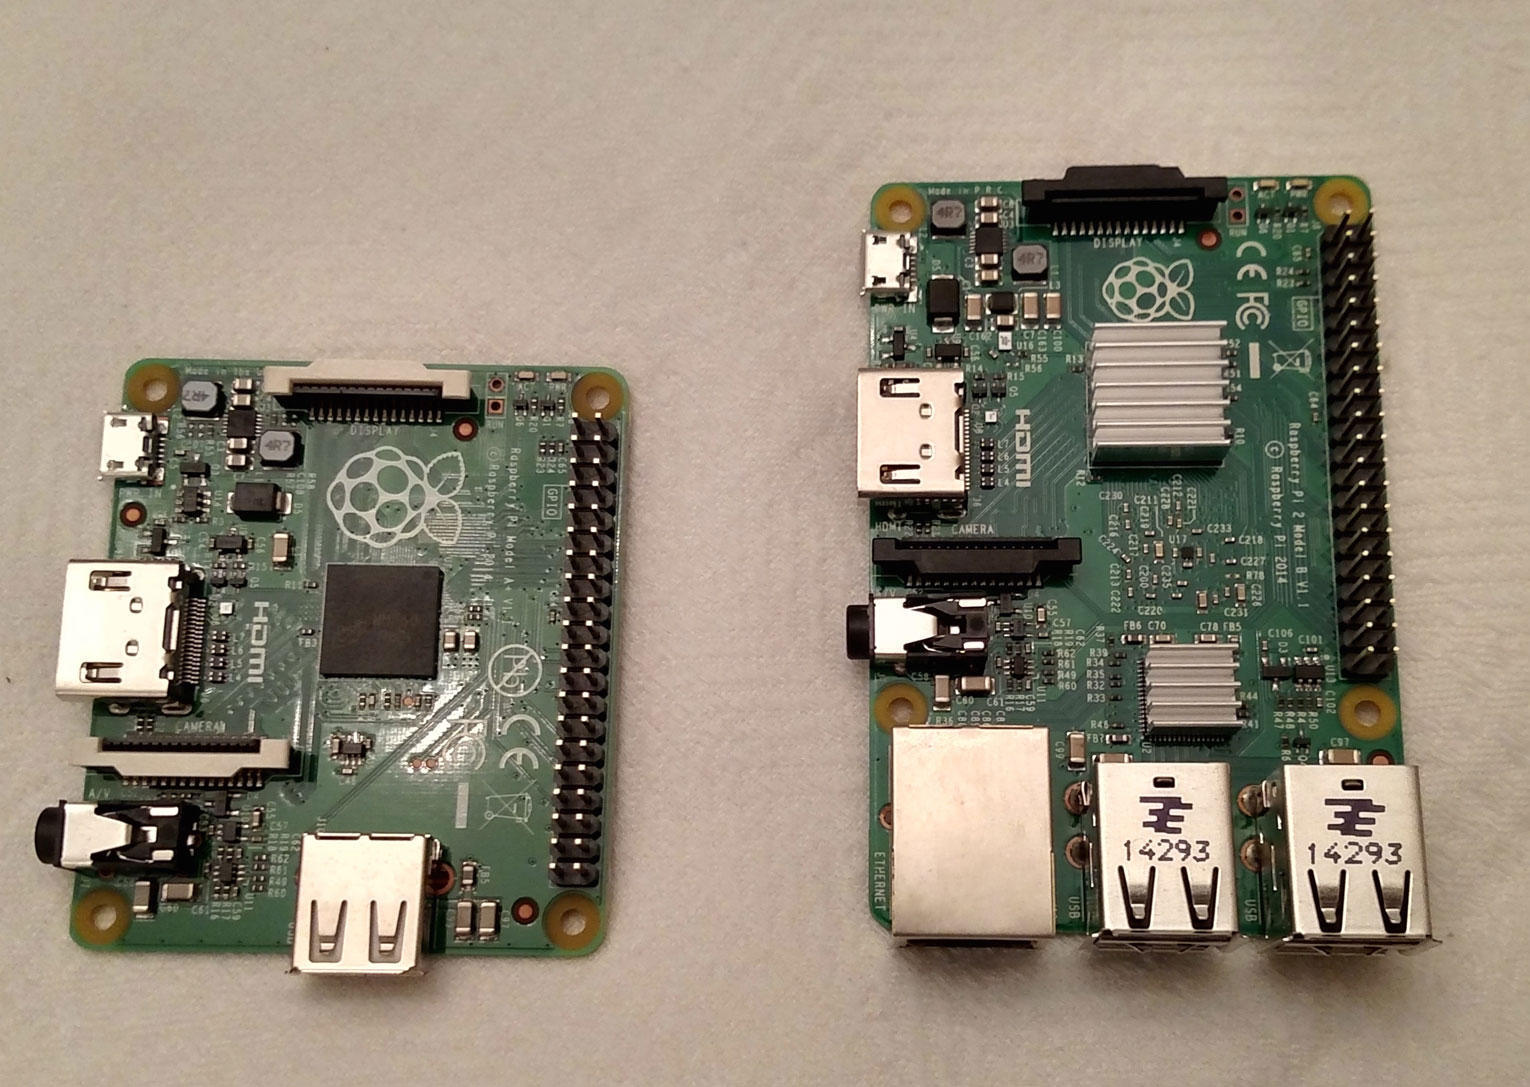
\includegraphics[width=0.6\textwidth]{img/rpia-rpi2b.jpg}
				\caption{\textit{Raspberry Pi} modelo A+ e \textit{Raspberry Pi} 2 modelo B.}
				\label{fig:rpia-rpi2b}
			}
		\end{figure}

Por ter uma comunidade grande e ativa, o seu estudo é facilitado. Um bom número de sites e comunidades estão desenvolvendo projetos com esse dispositivo e publicando suas conquistas. É possível encontrar tutoriais e passo-a-passo de um bom número de projetos, porém somente para aprendizado. Ao desenvolver um projeto mais elaborado isso pode servir como guia de estudo e aprofundamento.

As empresas tem investido um bom dinheiro na área de \textit{DIY} e \textit{IoT}. 



% ---

% ---
% Objetivos
% ---
\chapter{Objetivos}
% ---

% ---

% ---
\section{Objetivos Gerais}
% ---

O objetivo geral desse projeto é pesquisar sobre as tecnologias de \textit{beacons} e \textit{Raspberry Pi}, assim como suas dependências. Também é um objetivo desenvolver um protótipo de rastreador de \textit{beacons} utilizando o \textit{Raspberry Pi}.

% ---

% ---
\section{Objetivos Específicos}
% ---

\begin{alineas}
	\item Estudar o funcionamento de \textit{beacons} e \textit{Raspberry Pi}, assim como suas aplicações.
	\item Identificar os requerimentos básicos de funcionamento de \textit{beacons} e \textit{Raspberry Pi}.
	\item Definir os elementos para desenvolvimento do protótipo.
	\item Planejar a estrutura do sistema.
	\item Implementar o protótimo de acordo com a estrutura e elementos planejados.
\end{alineas}

% ---

% ---
% Método de Pesquisa
% ---
\chapter{Método de Pesquisa}
% ---

\lipsum[1]

% ---

% ---
% Fundamentação Teórica
% ---
\chapter{Fundamentação Teórica}
% ---

\lipsum[1]

% ---

% ---
% Cronograma
% ---
\chapter{Cronograma}
% ---

\lipsum[1]

% ---

% ----------------------------------------------------------
% Finaliza a parte no bookmark do PDF
% para que se inicie o bookmark na raiz
% e adiciona espaço de parte no Sumário
% ----------------------------------------------------------
%\phantompart

% ---
% Conclusão
% ---
%\chapter{Conclusão}
% ---

%\lipsum[1]

% ---


% ----------------------------------------------------------------------------------------------------------------------------------






% ----------------------------------------------------------
% ELEMENTOS PÓS-TEXTUAIS
% ----------------------------------------------------------
%\postextual
% ----------------------------------------------------------

% ----------------------------------------------------------
% Referências bibliográficas
% ----------------------------------------------------------
\bibliography{referencias}


%---------------------------------------------------------------------
% INDICE REMISSIVO
%---------------------------------------------------------------------
\phantompart
\printindex
%---------------------------------------------------------------------

}

\end{document}